\section{Reinforcement Learning for LLM Reasoning}

\subsection{Background}
\paragraph{Single-Turn Reinforcement Learning.}
Reinforcement Learning (RL) is a general framework to steer the behavior of LLMs by maximizing expected reward:
\begin{align*}
\mathbb{E}_{x \sim \mathcal{D},\, y \sim \pi_\theta(\cdot \mid x)}[R(x,y)],
\end{align*}
where $\mathcal{D}$ is a prompt distribution, $\pi_\theta$, is the LLM policy parameterized by $\theta$, and $R(x,y)$ is the reward for response $y$. Algorithms such as PPO~\citep{ppo,instructgpt} and GRPO~\citep{deepseekr1,deepseekmath} apply this objective to static datasets, yielding strong single-turn gains in math and code generation. 
% Full definitions are in the Supplementary.

\paragraph{Multi-Turn Extensions.}
Though these methods excel at optimizing a policy to produce a correct answer in a single attempt, real-world applications like tutoring, coding assistants, embodied agents demand \emph{multi-turn} interaction, where a model refines answers across steps under feedback. In domains like programming, automated feedback is readily available from compilers or unit tests, enabling iterative correction. But for tasks like mathematical reasoning, obtaining such dense feedback is difficult; often, only a final signal of correctness is available.

Recent work has begun addressing the challenge of sparse feedback in reasoning tasks by optimizing full interaction trajectories.
For example, CollabLLM~\citep{collabllm2025} introduces multi-turn fine-tuning with collaborative simulation and sparse rewards, while RAGEN~\citep{ragen} frames reasoning as an MDP to enable delayed credit assignment. However, these methods often depend on custom environments or simulated rewards, limiting scalability. Since most real-world math and code datasets are single-turn and collecting turn-level human feedback is costly, some efforts synthesize proxy signals~\citep{swegym, osworld} or build tool-augmented environments~\citep{searchr1, retool, mint}. Despite these workarounds, most training remains fundamentally grounded in single-turn RL paradigms.

These limitations give rise to a fundamental question:
\emph{Can models trained only with single-turn RL generalize to multi-turn reasoning?}

\begin{figure*}[t]
    \centering
    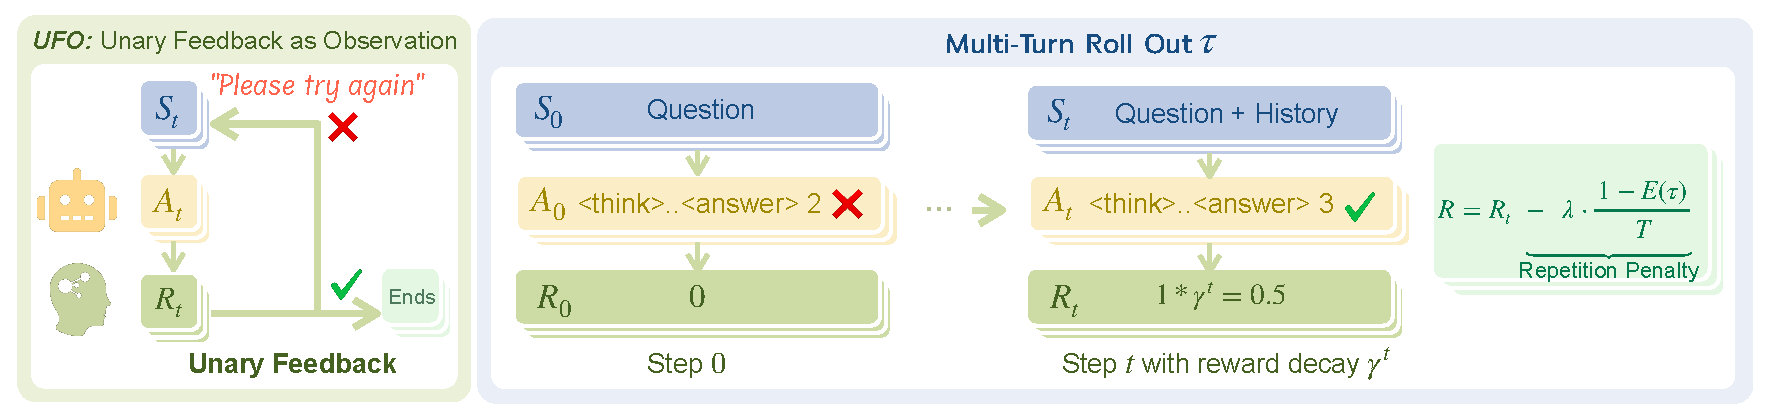
\includegraphics[width=0.98\linewidth]{figures/fig1.pdf}
    \vspace{10pt} 
    \caption{\textbf{The UFO framework for multi-turn training.} At each step $t$, the model observes the full interaction history and generates a response. Correct responses receive discounted rewards $\gamma^t$, while incorrect ones receive none. A repetition penalty based on the uniqueness of trajectory $\tau$ is applied after success or when the turn limit is reached.
    }
    \label{fig:ufo}
    % \vspace{-0.25cm}
\end{figure*}

\subsection{Single-Turn RL Leads to Collapsed Multi-Turn Reasoning}

To answer the question, we need to examine how models trained with single-turn RL perform in multi-turn setting. Practically, users typically offer minimal feedback (e.g., “try again”) and expect the model to adjust its reasoning accordingly. However, we find that single-turn RL models are \textbf{effective solvers but poor revisers}, consistently failing to incorporate feedback.

This phenomenon is illustrated in Figure~\ref{fig:example}: a pre-trained model refines its answer across turns, while a single-turn RL model fails to revise, repeating its initial output. To quantify this behavior, we use \emph{effective answer} as our metric, and the results were presented in Figure~\ref{fig:compare_unique} for off-the-shelf LLMs and Figure~\ref{fig:answer_repetition} for our trained models with single-turn RL. Empirically, after single-turn RL training, LLMs tend to give less effective answers across multiple turns.

Specifically, for off-the-shelf LLMs, we select models fine-tuned with various RL algorithms including PPO~\citep{ppo}, GRPO~\citep{deepseekmath}, DAPO~\citep{yu2025dapoopensourcellmreinforcement}, and Dr.\ GRPO~\citep{liu2025understanding}. Details of the models used can be found in the Appendix~\ref{sec:model-detail}. As shown in Figure~\ref{fig:compare_unique}, all models show a noticeable decrease in the unique answer ratio after RL training, and the extent varies by method and model size.
For example, under DAPO the effective answer ratio of the 32B model falls from 78.0\% to 65.7\%, and under Dr.\ GRPO that of the 1.5B model drops from 38.0\% to just 15.4\%. On the contrary, GRPO shows more moderate losses (e.g., the 0.5B model decreased from 34.0\% to 24.3\%), and the impact of PPO is also mild (the 7B model went from 57.6\% to 51.7\%). 
We also measure how many distinct answers our single-turn RL model provides for questions it fails to answer correctly for 5 consecutive turns (see Section~\ref{sec:exp_setup} for details). As shown in Figure~\ref{fig:answer_repetition}, under nearly 70\% cases the model provide identical wrong answers across multiple interaction turns.

\subsection{Theoretical Analysis}
\label{sec:theoretical_sketch}

We theoretically analyze why single-turn RL models tend to repeat mistakes in multi-turn settings. This behavior is a predictable consequence of the training process itself, which creates a \textbf{peaked, low-entropy output distribution}~\citep{cui2025entropymechanismreinforcementlearning, yue2025doesreinforcementlearningreally}. To quantify this tendency, we use the \emph{collision probability}, the likelihood that two independent samples are identical, which is formally defined as:
\begin{equation}
    \mathrm{Coll}(q) := \sum_y q(y \mid x)^2.
\end{equation}
This probability is fundamentally lower-bounded by the distribution's Shannon Entropy, $\mathcal{H}(q)$, as captured by the inequality:
\begin{equation}
    \mathrm{Coll}(q) \ge \exp(-\mathcal{H}(q)).
\end{equation}
We formalize this relationship with greater rigor and provide detailed proofs in Appendix~\ref{sec:app-repetition-theory}. This relationship proves that as a model's policy becomes more deterministic (lower entropy), the probability of repetition is forced to increase. For a static policy unable to learn from feedback, repetition is therefore an inevitable failure mode.

To overcome this limitation, a policy must be able to learn from its interaction history. We formalize this requirement using a Markov Decision Process (MDP) and define two distinct classes of policies. \textbf{Parallel Policies ($\Pi_{par}$)} correspond to traditional single-turn RL, where $k$ answers are sampled independently based only on the initial question. In contrast, \textbf{Sequential Policies ($\Pi_{seq}$)} make decisions based on the full history of interactions, allowing for adaptation after each failure. Since any parallel policy is a special case of a sequential one, it is clear that $\Pi_{par} \subseteq \Pi_{seq}$, and their expected success rates provably satisfy:
\begin{equation}
    \max_{\pi \in \Pi_{seq}} \mathbb{E}[\text{Succ@}k] \ge \max_{\pi \in \Pi_{par}} \mathbb{E}[\text{Succ@}k].
\end{equation}
This theoretical guarantee stems from the fact that a sequential policy can intentionally avoid previously known errors, thus increasing its subsequent conditional success probability. By Blackwell dominance~\citep{Blackwell1951}, its overall success rate is guaranteed to be at least as high as that of a parallel policy. We extend more detailed analysis in Appendix~\ref{app:theory-ufo}.

This highlights a critical gap: single-turn RL is insufficient for multi-turn reasoning. However, acquiring the necessary step-by-step supervision is often infeasible. In light of this, we ask the following question: \textbf{Can we leverage only the simplest form of supervision, such as “try again”, to simulate multi-turn interaction on static datasets and train models to learn adaptive revision behaviors?}
\begin{quote}
    \emph{Can minimal feedback alone unlock multi-turn reasoning on static datasets?}
\end{quote}

\section{Training Multi-Turn Reasoning Models with Unary Feedback}
\subsection{Problem Formulation}

We model the process of multi-turn problem solving based on static single-turn datasets as a finite-horizon Markov Decision Process (MDP), defined by the tuple $(\mathcal{S}, \mathcal{A}, \mathcal{P}, R, T_{\text{max}})$. Here, $\mathcal{S}$ is the state space, $\mathcal{A}$ is the action space consisting of all possible answers, $\mathcal{P}$ is the transition function defined by the agent–environment interaction, $R$ is the reward function, and $T_{\text{max}}$ is the maximum number of interaction steps per episode.
At each turn $t$, the agent observes a state $s_t \in \mathcal{S}$ that encodes the original question $q$ and the history of past attempts and feedbacks:
\begin{align}
    s_t = \texttt{Concat}(q, \{(a_k, f_k)\}_{k=1}^{t-1}),
\end{align}
where $a_k$ denotes the $k$-th answer, and $f_k$ is a feedback token returned by the environment. The agent then generates an answer $a_t \sim \pi_\theta(\cdot \mid s_t)$ and receives a scalar reward:
\begin{align}
    r_t = 
    \begin{cases}
        1, & \text{if } a_t \text{ is correct}, \\
        0, & \text{otherwise}.
    \end{cases}
\end{align}
The episode ends when the agent provides a correct answer or reaches the maximum number of steps $T_{\text{max}}$.
This formulation grounds the multi-turn learning problem in a standard RL framework.

\subsection{Unary Feedback as Observation (UFO)}

To implement the MDP described above on static datasets, we propose a simple yet general mechanism called \textbf{Unary Feedback as Observation (UFO)} (Figure~\ref{fig:ufo}). This mechanism defines how the state history is constructed and presented to the agent. The key idea is to restrict $f_k$ in the observation to negative signals only. Specifically, when an answer $a_k$ is incorrect, the feedback is a generic signal such as \texttt{TryAgain}. When the agent produces a correct answer, the episode terminates immediately. Consequently, no explicit positive confirmation (e.g., \texttt{Correct}) is ever added to the state history. The agent thus only receives unary feedback and must learn to revise its answers based solely on a history of failed attempts.

In practice, the prompt is constructed as a natural-language sequence concatenating all previous attempts and their feedback. For example:
\begin{quote}
\small
\texttt{Question: What is the value of ...? \\
Attempt 1: [wrong answer] \\
Feedback: Try Again. \\
...\\
Attempt K: [correct answer]}
\end{quote}

This UFO mechanism enables us to transform static single-turn datasets into multi-turn interaction episodes without requiring structural changes, expert annotations, or execution environments. Thus, UFO allows multi-turn RL on LLMs with minimal supervision.

\subsection{Reinforcement Learning with Unary Feedback}

Given the MDP formulation and the UFO-based observation design, we optimize the agent using RL to learn revision-aware and multi-turn policies. Since the dataset only contains the final-answer accuracy and lacks ground-truth reasoning traces, supervised finetuning is not applicable. Reinforcement learning, in contrast, enables exploration of diverse reasoning strategies under sparse and delayed supervision.

We adopt Proximal Policy Optimization (PPO) to train the policy $\pi_\theta$, following prior work~\citep{hu2025openreasonerzeroopensourceapproach, ragen} which shows that a learned critic enables fine-grained value estimates and stabilizes optimization.
At each episode, the agent interacts with a problem over multiple rounds. At each turn $t$, it observes input $x_t$, generates an answer $a_t$, and receives a binary reward $r_t \in \{0, 1\}$. The resulting trajectory is defined as:
\begin{align}
\tau = \{(x_1, a_1, r_1), (x_2, a_2, r_2), \dots, (x_T, a_T, r_T)\},
\end{align}
where $T \leq T_{\text{max}}$ is the number of turns before success or termination. The objective is to maximize the expected return:
\begin{align}
\mathcal{J}^{\text{RL}}(\theta) = \mathbb{E}_{\tau \sim \pi_\theta} \left[ \sum_{t=1}^{T} r_t \right].
\end{align}
We apply PPO with a clipped surrogate objective. For each training batch, we estimate the advantage $\hat{A}_t$ using a baseline value function and update the policy as:
\begin{align}
\mathcal{L}^{\text{PPO}}(\theta) = \mathbb{E}_t \left[ \min \left( \frac{\pi_\theta(a_t \mid x_t)}{\pi_{\theta_\text{old}}(a_t \mid x_t)} \hat{A}_t,\; \text{clip}(\frac{\pi_\theta(a_t \mid x_t)}{\pi_{\theta_\text{old}}(a_t \mid x_t)} \hat{A}_t, 1 - \epsilon, 1 + \epsilon) \right) \right].
\end{align}
Crucially, the UFO design enables the policy to condition on the full history of failure signals, giving rise to context-sensitive behaviors such as error correction, elimination, and hypothesis refinement—capabilities that are difficult to elicit through static supervision alone.

\subsection{Reward Design for Adaptive Reasoning}
\label{sec:reward_design}
Binary correctness signals offer a minimal form of supervision, but they could induce suboptimal behavior such as blind trial-and-error or repeated guesses. To encourage more efficient and reflective reasoning, we introduce a trajectory-level \textit{reward decay} with \textit{repetition penalty}. Reward decay encourages \textbf{minimality} by favoring trajectories that reach correct answers in fewer turns, thereby promoting concise and purposeful reasoning, while the repetition penalty promotes \textbf{diversity} by penalizing repetitive answers and encouraging the model to explore alternative reasoning strategies upon failure.

Formally, reward decay promotes early success by assigning exponentially diminishing rewards to correct answers produced at later turns:
\begin{align}
R_t = 
\begin{cases}
\gamma^t, & \text{if } a_t \text{ is correct}, \\
0, & \text{otherwise},
\end{cases}
\end{align}
where $\gamma \in (0, 1)$ is a decay factor that favors solving the problem in fewer turns.

We define the repetition penalty based on the number of \textit{effective answers}. Let $T$ denote the number of turns in the episode, and $E(\tau)$ be the number of effective answers in the trajectory $\tau$. We define a normalized penalty term:
\begin{align}
\text{Penalty}(\tau) = \lambda \cdot \left(1 - \frac{E(\tau)}{T} \right),
\label{eq:penalty}
\end{align}
where $\lambda > 0$ is a tunable penalty weight, and $E(\tau)/T$ measures answer diversity. The penalty is maximized when all answers are identical.

Combining above components, the trajectory-level reward for RL training is defined as:
\begin{align}
R =
R_t - \text{Penalty}(\tau).
\end{align}
To improve stability, we apply a small penalty $\eta < 0$ for each malformed or missing output across turns.
To summarize, the reward is determined by the reasoning correctness at the last turn, answer diversity and format correctness of model answers across turns. 

